\documentclass[12pt]{standalone}
\usepackage{tikz}
%\usetikzlibrary{calc, arrows.meta, decorations.pathreplacing}

\begin{document}

	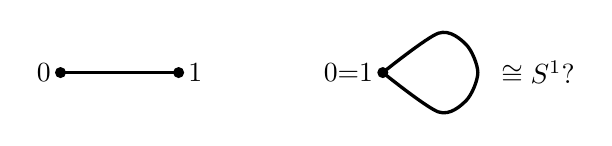
\begin{tikzpicture}
		\draw[very thick] (0,0) -- (1.5,0);
		\fill (0,0) circle (2pt) node[anchor=east]{0};
		\fill (1.5,0) circle (2pt) node[anchor=west]{1};
\begin{scope}[shift={(3.8, 0)}]
	\draw[very thick] plot[smooth] coordinates {(0.293, 0) (1, 0.5) (1.3535, 0.3535) (1.5, 0)  (1.3535, -0.3535) (1, -0.5)  (0.293, 0)};
	\fill (0.293,0) circle (2pt) node[anchor=east]{0=1};
	\node[anchor=west, xshift=5pt] at (1.5, 0) {$\cong S^1$?};
\end{scope}
\end{tikzpicture}
\end{document}
